The \fullcim (\cim) is a prototype of the \fullcis. The \cim consists of eight\footnote{The number of nodes is bounded by the hardware available to us.} battery-less intermittent nodes. Each node is capable of performing isolated word recognition. 
%
% The reason behind developing a \cim is threefold: (i) voice is a natural and convenient way for human to interact with miniaturized devices; (ii) demonstrating \textit{the world's first} battery-less intermittently-powered command recognizer, which shades light on the potential of battery-less intermittent systems; and (iii) facilitating testing with different sensing strategies and different type of external events arrival (i.e., regular  or burst). 

% Moreover, we believe that a \cim can facilitate direct human-to-human or human-to-objects communication. Imagine that a \cim based system is deployed in a play ground, embedded in ground and other objects. You want to call your child, and a \cim based system is embedded in your shirt and his shirt. You say his name and the \cim picks up the word and scatter it over light---\cite{marco}  demonstrates the feasibility of scattering sunlight to communicate between two nodes that are up to 60\,m apart. The scattered signal will be relied on other \cim nodes until the receiving node on his shirt receives the message and notify him, daddy is calling. 
%
\subsection{Hardware}
\label{sec:hardware}
A \cim node consists of thee main parts: a microphone, a MCU, and a harvester. MSP430RF5994~\cite{ti_msp430_website}, an ultra-low-power MCU, is used for data acquisition and processing. This MCU has a 16-bit RISC processor running on 1\,MHz, 8\,KB of SRAM (volatile), 256\,KB of FRAM (non-volatile), and a 12-bit analog to digital converter (ADC). It also features a Low Energy Accelerator (LEA), which offloads the main CPU for specific operations, such as FFT. For recording we use the PMM-3738-VM1010-R piezoelectric MEMS microphone, which features Wake on Sound and ZeroPower listening technologies \cite{microphone}, allowing both the MCU and the microphone to sleep in a low-power mode until a sound wave is detected.
The MCU and microphone are powered by a BQ25570 solar power harvester~\cite{BQ25570EVM-206_website} connected to an IXYS SLMD121H04L solar cell~\cite{SLMD121H04L_website} and a super-capacitor of 470 \si{\micro F}. For debugging we used the Saleae logic analyzer~\cite{saleae}.
%
\subsection{Software}
\label{sec:software}
The \cim runs power interrupts immune command recognizer. The recognizer is capable of recognizing isolated-word type of speech. 
The main parts of the recognizer are illustrated in Figure~\ref{fig:cis} and explained below:
%
\paragraph{Data acquisition}
The \textit{Wake-on-Sound} feature of the microphone triggers the data acquisition process once the energy level in the sound signal crosses a certain level. The ADC, then, samples the output of the microphone at 8\,kHz. This sampling rate is sufficient to cover most of the frequency range of the human voice. The recording length was set to 285\,ms, which suffices to get all the acoustic features needed to recognize the words.
% To determine the end of the recording we relied on the characteristics of the targeted vocabulary. In particular, we identified experimentally the minimum effective recording length, which is 
% 285\,ms for the chosen set of words. 
% By exploiting the Wake-on-Sound feature and using the minimum effective recording length, we eliminate the need for an endpoint detection algorithm, greatly improving the processing time and system efficiency from the energy perspective.
%
\paragraph{Feature Extraction}
For word recognition, we adopted the method presented in~\cite{hopper1992fft}. Here, we briefly describe the algorithm for convenience. The \cim starts by dividing the signal into frames of 256 samples ($\approx$ 33 milliseconds). 
Then, it computes a 256-point Fast Fourier Transform for each frame. The resulting feature vectors are normalized (by computing the binary logarithm of each entry of that vector) to reduce detection errors that result from differences in the amplitude of the speech input. This feature vectors are the basis for the word-identification process. 
%
\begin{figure}
	\centering
	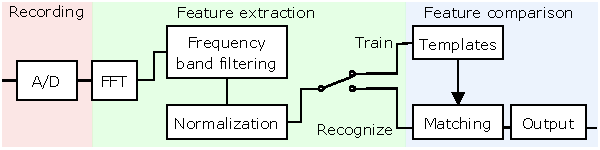
\includegraphics[width=\columnwidth]{figures/cis}
	\caption{The \fullCIM (\cim) features a power-failure-immune word recognizer. First, a word is recorded. Then, its spectral features are extracted. The resulting feature vector is compared against previously-stored words for recognition.}
	\label{fig:cis}
\end{figure}
%
\paragraph{Feature Matching}
Feature matching is achieved by computing the the squared Euclidean distance between the normalized feature vectors of the recorded word and the feature vectors of the words stored during the training phase (templates, see Table~\ref{tab:words}). 
% \cim computes the squared Euclidean distance between vectors of the record.
% as follows:
% \begin{equation}
% 	 	d_j = \sum\limits^S_{i=1} (f_{s,i} - f_{r,i})^2,
%     \label{eq:frame_dist}
% \end{equation}
% where $d_j$ is the distance between the $j^{\text{\tiny th}}$ stored and recorded vectors. 
% $f_{s,i}$ and $f_{r,i}$ are the normalized output of the $i^{\text{\tiny th}}$ spectral band of a stored and recorded vector, respectively.  
% % $f_{s,i}$ is the normalized output of the $i^{\text{\tiny th}}$ spectral band of a stored vector, $f_{r,i}$ is the normalized output of the $i^{\text{\tiny th}}$ spectral band of a recorded vector. 
% The total distance between two words is calculated as follows:
% \begin{equation}
% 		D_k = \sum\limits^{l}_{j=1} d(j)
% \end{equation}
% where $D_k$ is the distance between the $k^{\text{\tiny th}}$ stored word and the recorded word, and $l$ is the recording length measured in frames.
Once the recorded word has been compared to all template words, the template with the smallest distance to the recorded word is considered the correct word. However, if the smallest distance is bigger than a confidence threshold, then the \cim will return ``undefined word''. 

We have experimented with two feature matching algorithms: the Linear Distance Matching (LDM) and Dynamic Time Warping (DTW) algorithm. While LDM compares the feature vectors of two words successively, DTW looks for the minimum distance between the two vectors. In our implementation, the DTW was about 10 times slower than LDM, whereas the detection accuracy was comparable; therefore, we default our implementation to LDM.
%
% It should be emphasized that in the linear distance matching algorithm (LDM) the feature vectors of two words are compared successively, not accounting for differences in pronunciation speed. This is sufficient for our case as we are targeting isolated words and speaker dependent speech recognition type. We also implemented the Dynamic Time Warping algorithm which better handles the difference in the speed of speech. However, it is slower than the linear matching algorithm  (Table~\ref{tab:profiling}) and the detection accuracy was comparable in our case. Therefore, we default our implementation to LDM. 
%
\paragraph{Power-Failure Protection}
In order to preserve the progress state and to protect \cim data against randomly timed power failures, we split the recognition program into 19 atomic regions. 
We ensured that each of these regions requires less energy than what the energy buffer can provide with a single charge. 
The program state is checkpointed in non-volatile memory on the transition between these regions. This prevents the program from falling back to its starting point (\texttt{main()}) after each power failure. 
Data in non-volatile memory with Write-After-Read dependency is double-buffered to ensure data integrity when the power supply is interrupted.
%
\paragraph{Code profiling}
The entire command recognition software was written in {\tt C}. The total program consists of 973 lines of code, excluding the FFT function, which is imported from the Texas Instrument DSP library.
The memory footprint on the MCU is 20,064\,B of FRAM and 1,134\,B of SRAM.

The power usage of a node differs according to its activity. When a node is waiting for a voice event, it is in low-power mode. Recording a voice event activates the microphone, ADC and MCU (maximum power consumption). Processing the recorded data requires only the MCU to be on. Table~\ref{tab:power_usage} lists a node's power consumption for each of these states (sleeping, recording, and processing), as measured with a Monsoon power monitor~\cite{monsoon}. 
%
% When a signal is being recorded or processed, it is in active mode. When recording, the microphone and ADC consume additional power. The power consumption rates are determined by measuring the current with a Monsoon power monitor~\cite{monsoon} and shown in Table~\ref{tab:power_usage}.
%
% \begin{table}
% 	\centering
% 	\caption{Code statistics: lines of code}
% 	\label{tab:code_stats}
% 	%Compiled without optimization flags:
% 	\begin{tabular}{lrrrr} \hline
% 		Language & Files & Blank & Comment & Code \\\hline
% 		C & 7 & 264 & 173 & 736 \\
% 		C/C++ Header & 8 & 62 & 40 & 237 \\\hline
% 		Total &  15 & 326 & 213 & 973 \\\hline
% 	\end{tabular}
% \end{table}